\documentclass[12pt]{article}
\usepackage[top=1in, bottom=1in, left=1in, right=1in]{geometry}
\usepackage{paralist}
\usepackage{graphicx}
\usepackage{titlesec}  
\usepackage{amssymb}
\usepackage{amsmath} 
\usepackage{xcolor}

\begin{document}
\title{STAT 498 B Bootstrap}
\author{Nan Tang 1662478}
\date{\today}
\maketitle

\section*{Q1}
\begin{verbatim}
hist(incomes, breaks = 40, col = "skyblue")
mean(incomes) ##74106.03
sd(incomes) ##94039.74
quantile(incomes)
##      0%         25%         50%         75%        100% 
##2162.505   22058.828   45403.631   90048.464 1220475.923 
\end{verbatim}

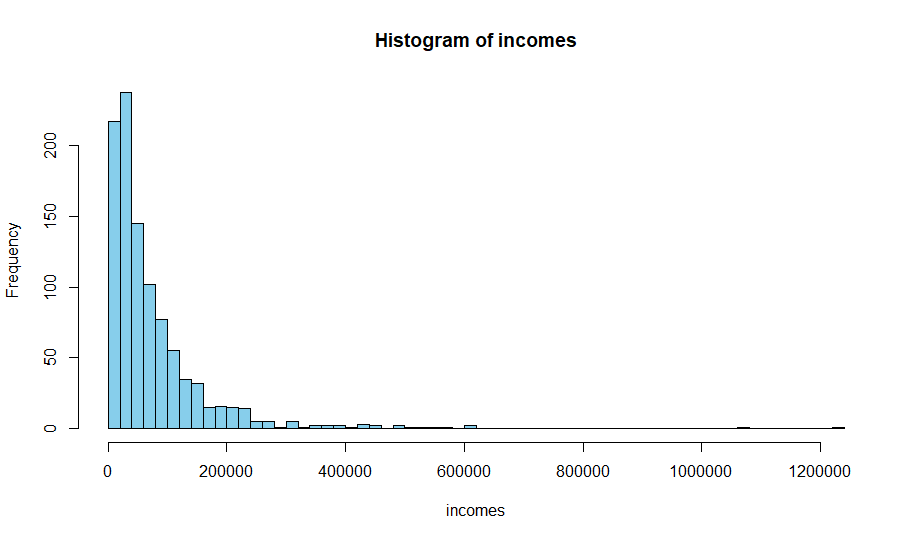
\includegraphics[width = 6.5 in]{Hist-incomes.png}

\noindent \textcolor{darkgray}{The histogram of incomes displayed an obvious skewed right distribution. From the relatively enormous standard deviation we can get that people's incomes vary largely in this country. One reason that causes the large sd is that there are several extreme values who earned over six hundred thousand per year.}

\section*{Q2}
\begin{verbatim}
topQuan <- quantile(incomes, prob=0.95) ##220665.7 
topSum <- sum(incomes[incomes > topQuan]) ##18689201
totalSum <- sum(incomes) ##74106034
topProp <- topSum / totalSum 
sprintf("%1.4f%%", 100*topProp) ##"25.2195%"
\end{verbatim}

\noindent \textcolor{darkgray}{We got that top 5$\%$ earner in this country owned 25.22$\%$ wealth among total income. If assuming everyone earns same money, top 5$\%$ people should earn 5$\%$ of total incomes.}

\section*{Q3}
\begin{verbatim}
kSimulation <- 10000
aSampleProp <- numeric(kSimulation)
for (i in 1 : kSimulation) {
  sample <- sample(incomes, length(incomes), replace=T)
  topQuan <- quantile(sample, prob=0.95)
  topSum <- sum(sample[sample > topQuan])
  aSampleProp[i] <- topSum / sum(sample)
}
CI.value <- quantile(aSampleProp, prob = c(0.025, 0.975)) ##0.2197676 ~ 0.2834287
hist(aSampleProp, breaks = 30, col = "skyblue", main = "Histogram of Top 5% 
Earners' Incomes Among Total Incomes")
abline(v = CI.value, lwd = 2, col = "orangered")
\end{verbatim}

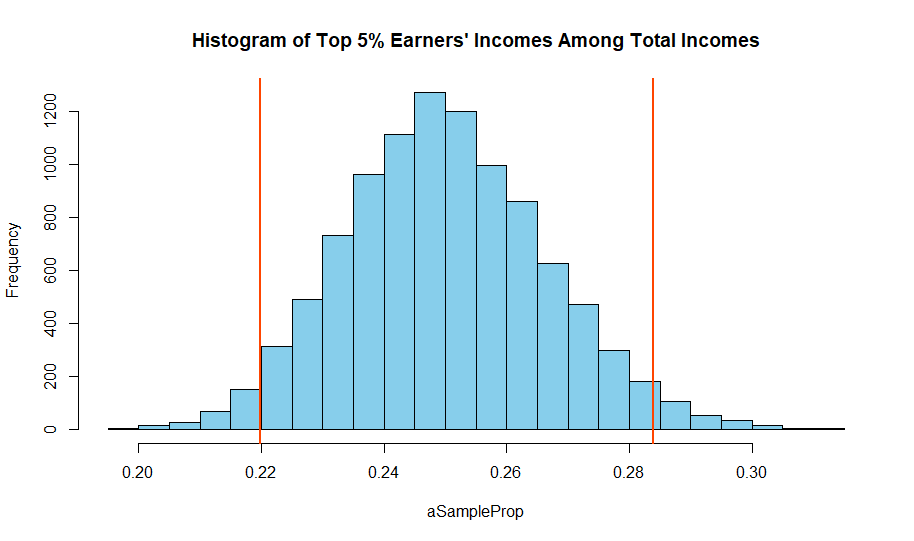
\includegraphics[width=6.5in]{Hist-top005.png}

\section*{Q4}
\begin{verbatim}
bSampleProp <- numeric(kSimulation) 
for (i in 1 : kSimulation) {
  sample <- sample(incomesB, length(incomesB), replace=T)
  topQuan <- quantile(sample, prob=0.95)
  topSum <- sum(sample[sample > topQuan])
  bSampleProp[i] <- topSum / sum(sample)
}
b.CI.value <- quantile(bSampleProp, prob = c(0.025, 0.975)) ##0.1849077 ~ 0.2276723

#Calculate 95% interval for difference between two populations.
prop.Diff <- numeric(kSimulation)
for (i in 1 : kSimulation) {
  prop.Diff[i] <- aSampleProp[i] - bSampleProp[i]
}
diff.CI <- quantile(prop.Diff, prob = c(0.025, 0.975)) ##0.00746182 ~ 0.08421688

#Calculate proportion of top 5% earner's income among total income.
bTopQuan <- quantile(incomesB, prob=0.95) 
bTopSum <- sum(incomesB[incomesB > bTopQuan]) 
bTotalSum <- sum(incomesB) 
bTopProp <- bTopSum / bTotalSum ##0.2068448

((topProp - bTopProp) > diff.CI[1]) && ((topProp - bTopProp) < diff.CI[2]) ##TRUE
\end{verbatim}

\noindent \textcolor{darkgray}{The difference in proportion between these two income samples falls in the confidence interval of 95$\%$, therefore, the difference is not statistically significant.}

\section*{Q5} 
\begin{verbatim}
diff.gini <- numeric(kSimulation)
for(i in 1 : kSimulation) {
  aSample <- sample(incomes, length(incomes), replace=T)
  bSample <- sample(incomesB, length(incomesB), replace=T)
  diff.gini[i] <- gini(aSample) - gini(bSample)
}
diff.gini.CI <- quantile(diff.gini, prob = c(0.05, 0.95)) ##0.04653538 ~ 0.10270242
\end{verbatim}

\noindent \textcolor{darkgray}{The 90$\%$ confidence interval of difference between two populations' gini coefficient is 0.0465 to 0.1027.}

\end{document}